\documentclass[twocolumn]{article}

%% Language and font encodings
\usepackage[english]{babel}
\usepackage[utf8]{inputenc}
\usepackage{csquotes}
\bibliographystyle{unsrt}
\usepackage{booktabs}

\usepackage{tabu}
\usepackage[T1]{fontenc}

%% Sets page size and margins
\usepackage[a4paper,top=2cm,bottom=2cm,left=3cm,right=3cm,marginparwidth=1.75cm]{geometry}

%% Useful packages
\usepackage{amsmath}
\usepackage{graphicx}
%\usepackage{apacite}
\usepackage[colorinlistoftodos]{todonotes}
\usepackage[colorlinks=true, allcolors=blue]{hyperref}

\title {{\it Project-} Support Vector machines (SVM) to build a Spam Classifier}
\author{B. Shadrack Jabes}
\date{\it{\today}}

\begin{document}
\maketitle

\section{Introduction}
Most of the email services today provide spam filters which classifies whether an email is spam or not?.
The aim of this project is to build a spam filter using SVMs.

\section{Dataset}
The dataset is an email that contains an URL, email address in the text, some numbers, symbols of money (dollars) and amount. Because the URLs or amount may be different and there is no unique way of representing them, I preprocess them  and replace it with some kind of unique strings. This improves the performance of the spam classifier.
	   \begin{figure}[htbp]
                \centering
                \includegraphics[clip=true,trim=0cm 0cm 0cm 0cm,width=8cm]{../sampleemail1.ps}\\
                \includegraphics[clip=true,trim=0cm 0cm 0cm 0cm,width=8cm]{../sampleemail2.ps}\\
                        \caption{Figure displays a sample email before and after preprocessing}
                \label{fig:dataset}
                \end{figure}

The preprocessing steps include the following simple steps:
\begin{itemize}
	\item Lower casing: Ignore capitalization of words
	\item stripping HTML tags: I remove the HTML tags leaving the contents
	\item replacing URLs: Now I replace the URLs with some string
	\item replacing amount: Numbers are replaced with text values
	\item replacing symbols of amount: All symbols are replaced with the text value
	\item replacing Email address: replacing email adress with text email address.
	\item word stemming: words that share similar word stems are replaced with just the stem keyword. For instance, 'discount', 'discounts', 'discounted', 'discounting' are all replaced with 'discount'.
	\item removing punctuations: remove non-words (like comma, semicolon, etc), punctuations.
\end{itemize}
The final processed form yields better SVM performance in extracting features and in building spam classifiers. A sample email before and after preprocessing is shown in figure \ref{fig:dataset}.
\section{Vocabulary list}
I have a list of words which is given as a part of the project. The list of words are collected by looking at the occurance of the words in spam corpus. For example   all words that  occur at least over 100 times in the spam corpus is stored.


Now I applied the vocabulary list to the preprocessed email text. So a particular word in the email is now mapped on to an index mentioned in the vocabulary list. If the word is not indexed in the vocabulary list then the word can be left unchanged.
\section{Feature extraction}
In this step each mail is converted into a vector with n dimensions. The feature vector $x$ is set to ones or zeros depending upon whether or not the $i^{th}$ word in the vocabulary present in email. The final array of $x$ will consist of an array with values either ones or zeros.
\section{Training SVM for spam classification}
The training set includes 4000 emails both spam and nonspam ones. The test set contains 1000 emails. Each of these emails are preprocessed and the features are extracted by following the recepie mentioned above. The code trains the SVM classifier to classify the emails and flags it spam (y = 1) or non spam (y =0)
\section{Contribution}
I implemented the vectorised SVM classifier to identify spam mails.
\end{document}
